\documentclass[sigconf,nonacm]{acmart}

\setcopyright{none}
\settopmatter{printacmref=false}
\renewcommand\footnotetextcopyrightpermission[1]{}
\pagestyle{plain}

\usepackage{booktabs}
\usepackage{tabularx}
\usepackage{array}
\usepackage{graphicx}
\usepackage{tikz}
\usetikzlibrary{shapes.geometric,arrows.meta,positioning,fit,backgrounds,calc}
\usepackage{url}
\urlstyle{rm}

%% ── Colours ──────────────────────────────────────────────────────────────────
\definecolor{cblue}  {RGB}{ 80,120,200}
\definecolor{cgreen} {RGB}{ 50,160, 80}
\definecolor{corange}{RGB}{210,120, 30}
\definecolor{cred}   {RGB}{200, 60, 50}
\definecolor{cgray}  {RGB}{100,100,100}
\definecolor{clb}    {RGB}{210,225,250}
\definecolor{clg}    {RGB}{205,240,210}
\definecolor{clo}    {RGB}{255,228,195}
\definecolor{clr}    {RGB}{255,215,210}
\definecolor{cyellow}{RGB}{255,245,180}

\title{Beyond Personal Data: Redefining Privacy in the Era of IoT, Operational
Technology, and Infrastructure-Level Data Protection}

\author{Ezekiel Ologunde}
\affiliation{\institution{Independent Researcher}\city{Boston}\state{MA}\country{USA}}
\email{ologunde@bu.edu}

\begin{abstract}
The traditional conceptualization of data privacy---focused primarily on protecting
personal information such as names, addresses, and financial records---proves
increasingly inadequate in hyperconnected industrial and critical infrastructure
environments. This paper examines how the October 2025 F5 Networks breach, wherein
nation-state actors exfiltrated source code and product configuration data, and the
Zscaler ThreatLabz 2025 report documenting surging cyberattacks against IoT and OT
devices, collectively illustrate a fundamental expansion in what constitutes
privacy-sensitive data requiring protection. Through analysis of contemporary threat
intelligence, nation-state targeting patterns of critical infrastructure, and the
architectural vulnerabilities inherent in legacy industrial systems retrofitted with
internet connectivity, we demonstrate that infrastructure-level data---including source
code, system architectures, sensor telemetry, process control parameters, and
operational patterns---presents privacy and security implications equivalent to or
exceeding traditional personal data. Our research reveals that many OT systems, designed
decades ago without cybersecurity considerations and subsequently connected to enterprise
networks, inadvertently expose sensitive operational data enabling adversaries to map
vulnerabilities and threaten critical infrastructure continuity. Through examination of
technical and non-technical controls addressing these expanded privacy requirements, we
propose an integrated framework encompassing data classification recognizing
infrastructure-level sensitivity, network segmentation, cryptographic protection, and
zero-trust architectures. The findings emphasize that modern privacy protection extends
beyond individual data subjects to encompass collective security---safeguarding the
integrity of systems serving entire populations.
\end{abstract}

\begin{CCSXML}
<ccs2012>
  <concept>
    <concept_id>10002978.10003006</concept_id>
    <concept_desc>Security and privacy~Privacy protections</concept_desc>
    <concept_significance>500</concept_significance>
  </concept>
  <concept>
    <concept_id>10002978.10003022</concept_id>
    <concept_desc>Security and privacy~Systems security</concept_desc>
    <concept_significance>500</concept_significance>
  </concept>
  <concept>
    <concept_id>10002978.10003014</concept_id>
    <concept_desc>Security and privacy~Software security engineering</concept_desc>
    <concept_significance>300</concept_significance>
  </concept>
</ccs2012>
\end{CCSXML}

\ccsdesc[500]{Security and privacy~Privacy protections}
\ccsdesc[500]{Security and privacy~Systems security}
\ccsdesc[300]{Security and privacy~Software security engineering}

\keywords{Privacy; data protection; IoT security; OT security; critical infrastructure;
industrial control systems; source code protection; nation-state threats; SCADA}

\begin{document}
\maketitle

%%──────────────────────────────────────────────────────────────────────────────
\section{Introduction}
%%──────────────────────────────────────────────────────────────────────────────

The contemporary discourse on data privacy has historically centered on protecting
personal information---names, addresses, financial records, health data, and behavioral
patterns of individual data subjects. Regulatory frameworks including the EU's GDPR,
California's CCPA, and HIPAA codify this person-centric paradigm, establishing
requirements for consent, data minimization, breach notification, and individual
rights~\cite{voigt2021gdpr}.

Two significant 2025 incidents illustrate how privacy has fundamentally expanded beyond
personal information to encompass infrastructure-level data whose compromise threatens
collective security and societal functioning. The October 2025 breach of F5
Networks~\cite{vincen2025f5,soper2025f5}, wherein nation-state actors exfiltrated source
code and product configuration data, and the Zscaler ThreatLabz 2025 report documenting
a sharp rise in attacks targeting IoT and OT devices in critical
sectors~\cite{zscaler2025threat}, collectively reveal that protecting data now means
protecting the very systems that keep contemporary society operational.

When adversaries compromise industrial control systems governing power generation, water
treatment, chemical manufacturing, or transportation infrastructure, the resulting harms
transcend individual privacy to threaten: (1)~\emph{public safety} through industrial
process manipulation causing mass casualties; (2)~\emph{economic stability} through
disruption of energy and logistics systems; (3)~\emph{national security} by enabling
adversaries to project power or degrade military capabilities; and (4)~\emph{societal
trust} through repeated infrastructure incidents eroding confidence in essential
services. This expanded threat landscape demands corresponding expansion in how we
conceptualize privacy and data protection.

\subsection{Research Questions and Contributions}

This paper addresses five critical questions: (RQ1)~How do IoT and OT security threats
differ from traditional IT challenges? (RQ2)~What infrastructure-level data categories
require protection equivalent to personal data? (RQ3)~How can organizations implement
controls protecting infrastructure data while maintaining operational efficiency?
(RQ4)~What policy frameworks are necessary for infrastructure data privacy?
(RQ5)~How must cybersecurity practice adapt to address collective security implications?

Our contributions include: (1)~analysis of the F5 breach and Zscaler report; (2)~
examination of unique OT security challenges and their privacy implications; (3)~a
framework for classifying infrastructure-level sensitive data; (4)~proposed technical
and non-technical controls; and (5)~discussion of how privacy conceptualization must
evolve.

%%──────────────────────────────────────────────────────────────────────────────
\section{Background and Related Work}
%%──────────────────────────────────────────────────────────────────────────────

\subsection{Traditional Privacy Frameworks}

Privacy as a legal and ethical concept has evolved significantly since Warren and
Brandeis defined it as ``the right to be let alone''~\cite{warren1890right}. Contemporary
scholarship recognizes multiple dimensions---informational, decisional, physical, and
associational privacy~\cite{solove2023understanding}. Privacy regulation has primarily
addressed informational privacy through principles of notice and consent, purpose
limitation, data minimization, security safeguards, and individual rights. However,
these frameworks assume harms primarily affect individual data subjects, an assumption
that breaks down when considering infrastructure-level data.

\subsection{Critical Infrastructure and Cybersecurity}

Critical infrastructure encompasses systems essential to societal functioning including
energy, water, transportation, healthcare, communications, and financial
services~\cite{cisa2023infrastructure}. Historically, operational technology existed in
isolated networks physically separated from enterprise IT---the ``air gap'' providing
inherent security through isolation~\cite{stouffer2023ot}. Business pressures for
efficiency and remote monitoring have driven IT-OT convergence, exposing previously
isolated industrial systems to cyber threats previously confined to IT
environments~\cite{lee2025dangerous}.

Many OT systems were designed 20--30 years ago without cybersecurity as a primary
concern~\cite{lee2025dragos}, exhibiting: lack of or weak authentication; unencrypted
communications; inability to support modern security software; embedded maintenance
credentials; vulnerability to network scanning; and inability to receive security
updates without extended downtime. When organizations connect these legacy systems to
networks without comprehensive security retrofitting, they create significant
vulnerabilities.

OT presents security challenges distinct from traditional IT: safety-critical operations
where failures can cause physical harm or loss of life; high availability requirements
preventing downtime for patching; real-time control constraints that security mechanisms
must not impair; proprietary protocols (Modbus, DNP3, PROFINET) that standard security
tools may not handle; 20--40 year operational lifespans; and scarce expertise combining
cybersecurity knowledge with industrial process understanding~\cite{stouffer2023ot}.

\subsection{Nation-State Threats to Critical Infrastructure}

Nation-state actors increasingly target critical infrastructure for espionage,
pre-positioning, and actual attacks. Stuxnet (2010) physically damaged Iranian nuclear
centrifuges through PLC manipulation~\cite{langner2023stuxnet}; Ukraine power grid
attacks (2015, 2016) caused widespread outages~\cite{case2021ukraine}; TRITON/TRISIS
(2017) targeted safety instrumented systems threatening catastrophic industrial
accidents~\cite{johnson2023triton}; and Volt Typhoon (2023--present) established
persistent access across U.S. critical infrastructure, apparently for
pre-positioning~\cite{cisa2024volt}.

\subsection{Supply Chain and Source Code Protection}

The F5 breach exemplifies supply chain risks. When adversaries compromise vendors
providing software or services to numerous downstream customers, they can potentially
affect thousands of organizations through a single breach~\cite{boyens2024supply}. Source
code theft enables: vulnerability discovery through code analysis; potential backdoor
insertion; intellectual property theft; and downstream risk to all customers whose
security depends on the compromised vendor's products.

%%──────────────────────────────────────────────────────────────────────────────
%% FIGURE 1 — Privacy Evolution (REDESIGNED)
%%
%% Three stacked layer boxes (5.0cm wide, centred) with left/right annotations.
%% Left annotation at x=−3.55 (text width 1.5cm) → left edge −4.30 cm  ✓
%% Right annotation at x=+3.55 (text width 1.5cm) → right edge +4.30 cm  ✓
%% Total figure width ≈ 8.6 cm  ✓  (column width ≈ 8.6 cm)
%%──────────────────────────────────────────────────────────────────────────────
\begin{figure}[h]
\centering
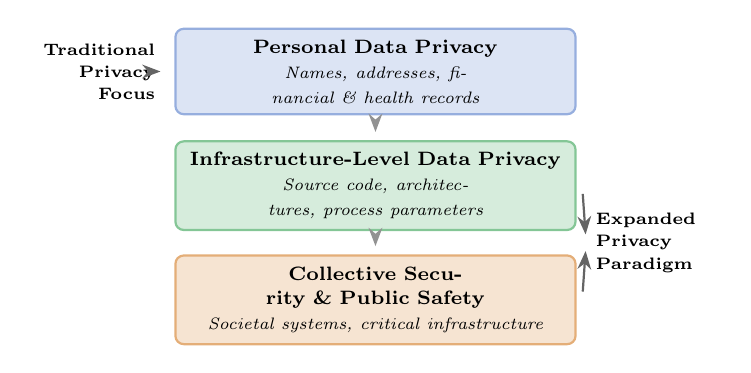
\begin{tikzpicture}[
  font=\fontsize{7pt}{9pt}\selectfont,
  >=Stealth,
  lyr/.style={
    rectangle, rounded corners=3pt,
    minimum width=5.0cm, minimum height=0.85cm,
    text centered, text width=4.8cm,
    draw, thick, inner sep=4pt
  },
  ann/.style args={#1}{
    font=\fontsize{6.5pt}{8pt}\selectfont,
    text width=1.5cm, align=#1
  },
  darr/.style={-{Stealth}, thick, dashed, cgray!70,
               shorten >=3pt, shorten <=3pt},
  sarr/.style={-{Stealth}, thick, cgray,
               shorten >=3pt, shorten <=3pt}
]
  %% ── Three layer boxes ────────────────────────────────────────────────────
  \node[lyr, fill=cblue!20,   draw=cblue!60]   (p1) at (0, 0.00)
    {\textbf{Personal Data Privacy}\\
     \fontsize{6.2pt}{7.5pt}\selectfont\itshape
     Names, addresses, financial \& health records};

  \node[lyr, fill=cgreen!20,  draw=cgreen!60]  (p2) at (0,-1.45)
    {\textbf{Infrastructure-Level Data Privacy}\\
     \fontsize{6.2pt}{7.5pt}\selectfont\itshape
     Source code, architectures, process parameters};

  \node[lyr, fill=corange!20, draw=corange!60] (p3) at (0,-2.90)
    {\textbf{Collective Security \& Public Safety}\\
     \fontsize{6.2pt}{7.5pt}\selectfont\itshape
     Societal systems, critical infrastructure};

  %% ── Downward flow arrows ────────────────────────────────────────────────
  \draw[darr] (p1.south) -- (p2.north);
  \draw[darr] (p2.south) -- (p3.north);

  %% ── Left annotation → top box ────────────────────────────────────────────
  \node[ann=right] (lbl) at (-3.55, 0.00)
    {\textbf{Traditional\\Privacy\\Focus}};
  \draw[sarr] (lbl.east) -- ([xshift=-2pt]p1.west);

  %% ── Right annotation ← from bottom two boxes ─────────────────────────────
  \node[ann=left] (rbl) at (3.55,-2.175)
    {\textbf{Expanded\\Privacy\\Paradigm}};
  \draw[sarr] ([xshift=2pt]p2.east) -- (rbl.west);
  \draw[sarr] ([xshift=2pt]p3.east) -- (rbl.west);
\end{tikzpicture}
\caption{Evolution of privacy protection: from a traditional focus on personal data
  toward an expanded paradigm encompassing infrastructure data and collective security.}
\label{fig:privacy_evolution}
\end{figure}

%%──────────────────────────────────────────────────────────────────────────────
\section{Case Study: F5 Networks Breach}
%%──────────────────────────────────────────────────────────────────────────────

In October 2025, F5 Networks disclosed that nation-state actors had breached its internal
systems and exfiltrated portions of source code and product configuration
data~\cite{vincen2025f5}. F5 products provide application delivery controllers, web
application firewalls, and network security services deployed by thousands of
organizations globally, including many critical infrastructure
operators~\cite{soper2025f5}. Attribution pointed to Chinese APT groups, consistent with
patterns of operations targeting technology companies to acquire intellectual property
and identify vulnerabilities in widely-deployed products.

The breach involved: \emph{source code} enabling adversaries to identify exploitable
vulnerabilities; \emph{product configuration data} revealing customer deployment patterns
and security configurations; and \emph{internal system data} about F5's development and
production environments. While involving no traditional personal data, the security
implications are profound: a single vulnerability discovered in stolen F5 source code
could be exploited across thousands of customer networks globally, including critical
infrastructure relying on F5 products for network security.

\begin{table}[h]
\caption{Personal Data vs.\ Infrastructure-Level Data Breaches Compared.}
\label{tab:comparison}
\small
\begin{tabularx}{\columnwidth}{@{}p{1.9cm}XX@{}}
\toprule
\textbf{Aspect} & \textbf{Personal Data} & \textbf{Infrastructure Data} \\
\midrule
Primary Harm     & Individual privacy, identity theft & Collective security, public safety \\
\addlinespace[3pt]
Affected Parties & Specific data subjects             & Entire populations, regions \\
\addlinespace[3pt]
Regulatory Frame & GDPR, CCPA, HIPAA                  & Limited specific regulation \\
\addlinespace[3pt]
Notification     & Individual required                 & No clear requirements \\
\addlinespace[3pt]
Remediation      & Credit monitoring, identity protection & Vulnerability patching, hardening \\
\addlinespace[3pt]
Long-term Risk   & Financial fraud, discrimination    & Infrastructure disruption, nat.\ security \\
\bottomrule
\end{tabularx}
\end{table}

Key lessons from the F5 breach: source code is a high-value nation-state target enabling
downstream exploitation; vendor breaches create systemic risk across thousands of
customers; traditional privacy frameworks are insufficient for infrastructure data whose
security implications exceed many personal data breaches in severity; and organizations
whose products secure critical infrastructure have particular obligations to transparently
disclose incidents affecting product security.

%%──────────────────────────────────────────────────────────────────────────────
\section{The IoT and OT Threat Landscape}
%%──────────────────────────────────────────────────────────────────────────────

\subsection{Zscaler ThreatLabz 2025 Key Findings}

The Zscaler ThreatLabz 2025 report documented a sharp rise in cyberattacks targeting
IoT and OT devices~\cite{zscaler2025threat}. Attack volume increases reflect growing
attacker awareness of IoT/OT vulnerabilities, increasing availability of specialized
attack tooling, higher-value targets as more critical systems connect to networks, and
relatively weak defenses in many IoT/OT environments. Attacks disproportionately
targeted energy, manufacturing, water treatment, and transportation infrastructure.
Common techniques included exploitation of known vulnerabilities, brute-force against
default credentials, network reconnaissance, man-in-the-middle against unencrypted
industrial protocols, and ransomware specifically targeting industrial environments.

\subsection{Operational Data as Privacy-Sensitive Information}

When adversaries compromise IoT and OT systems, they gain access to operational data
that, while not containing personal information, has significant security implications.
Industrial sensor telemetry (temperature, pressure, flow rates, power consumption)
reveals system capacity and operational margins, normal patterns enabling anomaly
detection avoidance, and vulnerability windows during process transitions. Process
control parameters specify safe operating limits, emergency shutdown thresholds, control
algorithms, and interlocks---information enabling adversaries to identify parameters that
if manipulated could cause unsafe conditions, and to develop attacks evading or disabling
safety systems. Energy usage patterns from smart meters and industrial monitoring reveal
facility occupancy, production schedules, and critical load dependencies.

\subsection{Legacy Systems and Retrofit Vulnerabilities}

Many current industrial systems were designed in the 1990s and early 2000s when security
assumptions included physical isolation providing inherent security, controlled facility
access preventing tampering, and protocol obscurity hindering attacks. These assumptions
no longer hold when systems connect to enterprise networks or the
internet~\cite{lee2025dragos}. Securing legacy OT presents significant challenges: many
systems cannot be patched without extended downtime; adding security mechanisms may
impact real-time performance requirements; modern security tools may not support legacy
protocols; and testing security changes in production industrial environments risks
costly disruptions~\cite{fortinet2025ot}.

%%
%% FIGURE 2 — IT / IoT / OT system types (two-column span)
%%
%% Three actor boxes (5.5cm wide each, gap 0.6cm) side-by-side = 17.7cm total.
%% Threat banner spans full width at top.
%% Total width ≈ 17.7 cm  ✓  (textwidth ≈ 17.8 cm for figure*)
%%
\begin{figure*}[t]
\centering
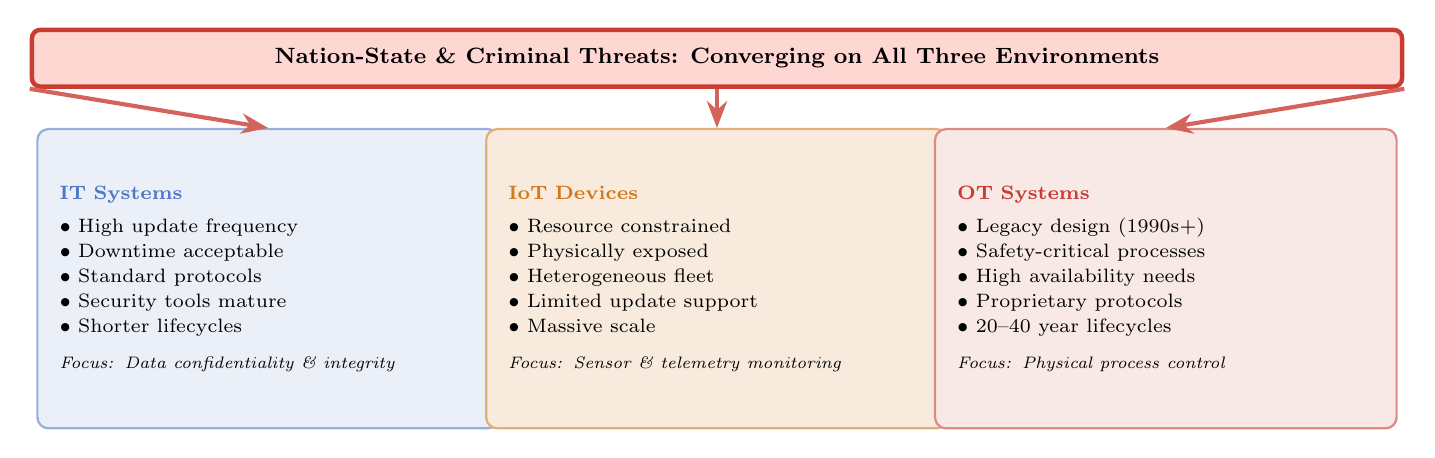
\begin{tikzpicture}[
  font=\fontsize{7pt}{9pt}\selectfont,
  >=Stealth,
  sys/.style={
    rectangle, rounded corners=4pt,
    minimum width=5.5cm, minimum height=3.8cm,
    text width=5.3cm, align=left,
    draw, thick, inner sep=8pt
  },
  thr/.style={
    rectangle, rounded corners=3pt,
    minimum width=17.4cm, minimum height=0.72cm,
    text centered, draw=cred, ultra thick,
    fill=clr, font=\fontsize{8pt}{10pt}\selectfont\bfseries
  },
  arr/.style={-{Stealth}, line width=1.5pt}
]
  %% ── Three system boxes ───────────────────────────────────────────────────
  \node[sys, fill=cblue!12, draw=cblue!60] (it) at (-5.7, 0) {
    \textbf{\textcolor{cblue}{IT Systems}}\\[3pt]
    $\bullet$ High update frequency\\
    $\bullet$ Downtime acceptable\\
    $\bullet$ Standard protocols\\
    $\bullet$ Security tools mature\\
    $\bullet$ Shorter lifecycles\\[4pt]
    \textit{\fontsize{6pt}{7.5pt}\selectfont Focus: Data confidentiality \& integrity}
  };

  \node[sys, fill=corange!15, draw=corange!60] (iot) at (0, 0) {
    \textbf{\textcolor{corange}{IoT Devices}}\\[3pt]
    $\bullet$ Resource constrained\\
    $\bullet$ Physically exposed\\
    $\bullet$ Heterogeneous fleet\\
    $\bullet$ Limited update support\\
    $\bullet$ Massive scale\\[4pt]
    \textit{\fontsize{6pt}{7.5pt}\selectfont Focus: Sensor \& telemetry monitoring}
  };

  \node[sys, fill=cred!12, draw=cred!60] (ot) at (5.7, 0) {
    \textbf{\textcolor{cred}{OT Systems}}\\[3pt]
    $\bullet$ Legacy design (1990s+)\\
    $\bullet$ Safety-critical processes\\
    $\bullet$ High availability needs\\
    $\bullet$ Proprietary protocols\\
    $\bullet$ 20--40 year lifecycles\\[4pt]
    \textit{\fontsize{6pt}{7.5pt}\selectfont Focus: Physical process control}
  };

  %% ── Threat banner above ──────────────────────────────────────────────────
  \node[thr] (thr) at (0, 2.8)
    {Nation-State \& Criminal Threats: Converging on All Three Environments};

  %% ── Arrows from banner to boxes ──────────────────────────────────────────
  \draw[arr, color=cred!80] (thr.south west) -- (it.north);
  \draw[arr, color=cred!80] (thr.south)      -- (iot.north);
  \draw[arr, color=cred!80] (thr.south east) -- (ot.north);

\end{tikzpicture}
\caption{Three system categories (IT, IoT, OT) with distinct security characteristics
  facing converging threats. IT-OT convergence exposes legacy operational systems to
  threats previously confined to IT environments.}
\label{fig:system_types}
\end{figure*}

%%──────────────────────────────────────────────────────────────────────────────
\section{Rethinking Privacy for Infrastructure Data}
%%──────────────────────────────────────────────────────────────────────────────

\subsection{Infrastructure-Level Data Categories}

Several categories of infrastructure-level data require privacy protection equivalent
to personal data. \textbf{Source code and software artifacts}---as demonstrated by
F5---enable adversaries to discover vulnerabilities and affect all downstream
deployments. \textbf{System architectures and network designs} reveal system
interdependencies, potential single points of failure, access paths, and segmentation
boundaries. \textbf{Operational parameters and process control data} including setpoints,
control algorithms, and safety limits enable understanding of how to manipulate systems
and identify unsafe operating regions. \textbf{Sensor and telemetry data} provides
insight into normal operating patterns and timing information for coordinated attacks.
\textbf{Product configuration and deployment data} reveals security control
effectiveness, common deployment weaknesses, and customer-specific configurations.

\subsection{Threat Models for Infrastructure Data}

Nation-state actors target infrastructure data for pre\-positioning in critical
infrastructure for potential future disruption, strategic intelligence about adversary
capabilities, technology transfer stealing intellectual property, and operational
planning enabling targeted attacks. Criminal actors increasingly target OT for
ransomware, extortion threatening safety incidents, stolen operational data for sale,
and sabotage-for-hire.

\subsection{Privacy Harms Beyond Individual Impact}

Infrastructure data breaches create harms fundamentally different from traditional
privacy violations. \emph{Collective security degradation} affects entire populations
dependent on compromised systems rather than specific individuals. \emph{Public safety
risks} arise from manipulation of industrial processes, safety systems, or critical
infrastructure causing physical destruction, toxic releases, or cascading infrastructure
failures. \emph{Economic disruption} through production losses, supply chain disruptions,
and recovery costs extends across entire industries. \emph{Erosion of trust} in essential
services, infrastructure operators, and government protective capacity creates lasting
societal harm. \emph{National security implications} arise when infrastructure
compromises degrade military capabilities or enable adversarial coercion.

%%──────────────────────────────────────────────────────────────────────────────
\section{Integrated Protection Framework}
%%──────────────────────────────────────────────────────────────────────────────

\subsection{Non-Technical Controls}

\textbf{Data Classification.} Organizations must expand classification beyond personal
data to include: \emph{Critical Infrastructure Data} whose compromise directly threatens
safety; \emph{Operational Technology Data} including process parameters and control
configurations; \emph{Architecture and Design Data} comprising network topologies and
security designs; \emph{Source Code and Intellectual Property}; and \emph{Deployment and
Configuration Data}. Each category requires defined sensitivity levels, access policies,
handling requirements, retention schedules, and breach notification obligations.

\textbf{Third-Party Risk Management.} Given supply chain risks demonstrated by F5:
assess vendor security practices before procurement; include security requirements in
contracts; require breach notification for vendor incidents; maintain vendor criticality
ratings; conduct periodic vendor security reviews; and plan for vendor compromise
scenarios~\cite{boyens2024supply}.

\textbf{Security Awareness.} Personnel handling infrastructure data require specialized
training on infrastructure data sensitivity, recognizing social engineering targeting
operational data, proper handling procedures, and the public safety consequences of data
compromise.

\subsection{Technical Controls}

\textbf{Network Segmentation.} Fundamental defense separating OT from enterprise IT
through defense-in-depth architecture (field devices → operations/control → business
logistics → enterprise IT), firewalls between IT and OT networks, unidirectional
gateways for critical data flows, and microsegmentation within OT zones. Access control
should minimize IT-OT connections, require MFA for OT access, enforce least-privilege,
and route remote access through jump hosts with full logging.

\textbf{Encryption.} Cryptographic protection for data at rest (full-disk encryption,
HSM-protected keys, key rotation); data in transit (TLS/SSL, VPNs for remote access,
endpoint authentication); and source code (encrypted repositories, signed commits,
access controls, code exfiltration monitoring).

\textbf{Continuous Monitoring.} Industrial network monitoring tools establishing normal
traffic baselines and detecting anomalous communications; centralized logging of access
to sensitive data; behavioral analytics identifying unusual access patterns and insider
threat indicators; and SIEM correlation across IT and OT environments.

\textbf{Zero Trust Architecture.} Verify explicitly (authenticate all access, validate
device posture, consider contextual risk); enforce least privilege (minimum necessary
permissions, just-in-time access, regular access reviews); and assume breach (minimize
blast radius through segmentation, monitor for lateral movement, maintain offline backups
for recovery).

\begin{table*}[t]
\caption{Technical and Non-Technical Controls for Infrastructure Data Protection.}
\label{tab:controls}
\small
\setlength{\tabcolsep}{5pt}
\begin{tabularx}{\textwidth}{@{}p{3.0cm}XX@{}}
\toprule
\textbf{Control Category} & \textbf{Non-Technical Controls} & \textbf{Technical Controls} \\
\midrule
Data Classification  & Classification schemes, policies, data ownership & Automated labeling, DLP policies \\
\addlinespace[3pt]
Access Control       & Authorization policies, approval workflows        & Authentication, RBAC, PAM \\
\addlinespace[3pt]
Segmentation         & Policies defining IT/OT boundaries                & Firewalls, VLANs, unidirectional gateways \\
\addlinespace[3pt]
Monitoring           & Procedures, escalation processes                  & SIEM, industrial network monitoring, UEBA \\
\addlinespace[3pt]
Encryption           & Key management policies, retention schedules      & Encryption at rest and in transit \\
\addlinespace[3pt]
Incident Response    & Playbooks, communication plans, regulator contacts & Forensic tools, automated containment \\
\addlinespace[3pt]
Third-Party Risk     & Vendor assessment, contract requirements          & Vendor access monitoring, SBOMs \\
\addlinespace[3pt]
Training             & Awareness programs, tabletop exercises            & Phishing simulation, testing \\
\bottomrule
\end{tabularx}
\end{table*}

%%──────────────────────────────────────────────────────────────────────────────
\section{Policy and Regulatory Considerations}
%%──────────────────────────────────────────────────────────────────────────────

\subsection{Current Regulatory Gaps}

Existing privacy regulations focus on personal data, creating gaps for infrastructure
data. Breach notification requirements typically apply only to personal data compromises.
Mandatory data protection controls often apply only to personal data. Individual rights
(access, correction, deletion) presume individual data subjects. Privacy regulators may
lack expertise in industrial cybersecurity. Sector-specific regulations (NERC CIP for
electrical, TSA Security Directives for pipelines, EPA water sector requirements, FDA
medical device guidance) focus on operational security rather than data protection
specifically. CISA's CIRCIA requires reporting substantial cyber incidents within 72
hours but focuses on incidents rather than data protection.

\subsection{Recommended Policy Enhancements}

\textbf{Expand Breach Notification.} Define infrastructure data categories requiring
notification; establish disclosure timelines to sector regulators and CISA; mandate
customer notification for vendor breaches; and require public disclosure when public
safety is implicated.

\textbf{Data Protection Standards.} Establish baseline controls for infrastructure
data including mandatory encryption, network segmentation requirements, authentication
standards, monitoring and logging requirements, and regular security assessments.

\textbf{Vendor Accountability.} Due diligence requirements for critical infrastructure
vendors; liability frameworks for vendor breaches affecting customers; mandatory security
standards and independent audits; and transparency obligations about security practices
and incidents.

\textbf{Information Sharing.} Legal protections for threat intelligence sharing;
sector-specific ISACs with government participation; anonymized incident data sharing;
classified briefings on nation-state threats; and international cooperation on
infrastructure protection.

%%──────────────────────────────────────────────────────────────────────────────
\section{Conclusion}
\sloppy
%%──────────────────────────────────────────────────────────────────────────────

The October 2025 F5 Networks breach and the Zscaler ThreatLabz 2025 report illustrate a
fundamental truth: data privacy has expanded far beyond personal information to encompass
infrastructure-level data whose protection is essential to collective security and
societal functioning.

Five key findings emerge. The \emph{privacy paradigm must shift} beyond individual data
subjects to encompass source code, system architectures, operational parameters, and
process control data threatening collective security when compromised. \emph{Legacy OT
vulnerabilities} created by decades-ago designs and subsequent internet connectivity
create systemic exposure that adversaries increasingly exploit~\cite{lee2025dragos}.
\emph{Supply chain systemic risk} means single vendor compromises like F5 can cascade
across thousands of downstream customers, including critical infrastructure operators.
\emph{Regulatory gaps} in current personal-data-focused frameworks leave infrastructure
data protection inadequately addressed. \emph{Integrated controls} spanning technical
segmentation, encryption, and monitoring with non-technical classification, training,
and vendor management are collectively required.

Perhaps most fundamentally, these cases demonstrate that cybersecurity in the
infrastructure context is inherently about \emph{collective security}. When adversaries
steal F5 source code, they potentially endanger thousands of organizations and millions
of people. When attackers compromise energy or water infrastructure control systems, they
threaten public safety for entire communities. When nation-states pre-position in
critical infrastructure networks, they create strategic vulnerabilities affecting
national security.

Protecting infrastructure data is not merely preventing unauthorized access---it is
preserving trust in the systems that modern civilization depends upon. This is the
expanded privacy paradigm that the contemporary threat landscape demands, and it is the
responsibility of cybersecurity professionals, organizational leaders, and policymakers
to implement.

%%──────────────────────────────────────────────────────────────────────────────
\sloppy
\bibliographystyle{ACM-Reference-Format}
\begin{thebibliography}{18}

\bibitem{zscaler2025threat}
Zscaler ThreatLabz. 2025. \textit{State of IoT and OT Security Report 2025}. Zscaler.
\url{https://www.zscaler.com/resources/industry-reports/threatlabz-mobile-iot-ot-report.pdf}

\bibitem{vincen2025f5}
A.J.~Vincen and R.~Satter. 2025. Breach at U.S.-based cybersecurity provider F5 blamed
on China. \textit{Reuters}.
\url{https://www.reuters.com/technology/breach-us-based-cybersecurity-provider-f5-blamed-china}

\bibitem{soper2025f5}
T.~Soper. 2025. F5 discloses major security breach linked to nation-state hackers.
\textit{GeekWire}.
\url{https://www.geekwire.com/2025/f5-discloses-major-security-breach-linked-to-nation-state-hackers/}

\bibitem{lee2025dragos}
R.~M.~Lee. 2025. Dragos' Lee says industrial systems unprepared for modern cyber threats.
\textit{Industrial Cyber}.
\url{https://industrialcyber.co/industrial-cyber-attacks/dragos-lee-says-industrial-systems-unprepared}

\bibitem{lee2025dangerous}
R.~M.~Lee. 2025. A dangerous blind spot in infrastructure cybersecurity.
\textit{World Economic Forum}.
\url{https://www.weforum.org/stories/2025/10/dangerous-blindspot-in-infrastructure-cybersecurity/}

\bibitem{fortinet2025ot}
Fortinet. 2025. \textit{2025 State of Operational Technology and Cybersecurity Report}.
\url{https://www.waterisac.org/wp-content/uploads/2025/08/FORTINET-2025-State-of-Operational-Technology-and-Cybersecurity-Report.pdf}

\bibitem{voigt2021gdpr}
P.~Voigt and A.~von dem Bussche. 2021. \textit{The EU GDPR: A Practical Guide}.
Springer.

\bibitem{solove2023understanding}
D.~J.~Solove. 2023. \textit{Understanding Privacy}. Harvard University Press.

\bibitem{warren1890right}
S.~D.~Warren and L.~D.~Brandeis. 1890. The Right to Privacy.
\textit{Harvard Law Review} 4, 5, 193--220.

\bibitem{cisa2023infrastructure}
CISA. 2023. Critical Infrastructure Sectors. U.S. Department of Homeland Security.

\bibitem{stouffer2023ot}
K.~Stouffer, J.~Falco, and K.~Scarfone. 2023. \textit{Guide to Operational Technology
(OT) Security} (SP 800-82 Rev.~3). NIST.

\bibitem{stellios2021survey}
I.~Stellios et al. 2021. A Survey of IoT-Enabled Cyberattacks.
\textit{IEEE Commun.\ Surveys Tut.} 23, 1, 233--274.

\bibitem{langner2023stuxnet}
R.~Langner. 2023. \textit{To Kill a Centrifuge: A Technical Analysis of Stuxnet}.
Langner Group.

\bibitem{case2021ukraine}
R.~M.~Case. 2021. Analysis of the Cyber Attack on the Ukrainian Power Grid. E-ISAC.

\bibitem{johnson2023triton}
S.~Caltagirone, A.~Pendergast, and C.~Betz. 2023. \textit{TRISIS Malware: Analysis of
Safety System Targeted Malware}. Dragos.

\bibitem{turton2021colonial}
W.~Turton and K.~Mehrotra. 2021. Hackers Breached Colonial Pipeline Using Compromised
Password. \textit{Bloomberg}.

\bibitem{cisa2024volt}
CISA. 2024. PRC State-Sponsored Actors Compromise and Maintain Persistent Access to
U.S. Critical Infrastructure. Advisory AA23-144A.

\bibitem{boyens2024supply}
J.~M.~Boyens et al. 2024. \textit{Cybersecurity Supply Chain Risk Management Practices}
(SP 800-161 Rev.~1). NIST.

\end{thebibliography}

\end{document}
